
\section*{Общая характеристика работы}

%\newcommand{\actualitySynopsis}{\underline{\textbf{\actualityTXT}}}

% \underline{\textbf{\actualityTXT}} Теория массового обслуживания (ТМО) занимается построением и анализом моделей для сложных систем, осуществляющих большое количество однотипных операций по обслуживанию различного рода требований (заявок). Первые работы в этой области были мотивированы решением прикладных задач, связанных с организацией деятельности телефонных станций в начале XX века. Задачи, поставленные и рассмотренные Ф.В.~Йоханнсеном и А.К.~Эрлангом, заложили основу для так называемой классической ТМО. Дальнейшее развитие этой отрасли науки связано с именами таких ученых как Ф.~Поллачек, А.Н.~Колмогоров, А.Я.~Хинчин, Б.В.~Гнеденко, И.Н.~Коваленко, К.~Пальм, Д.Дж.~Кендалл, Л.~Такач, Д.Р.~Кокс, У.Л.~Смит, Т.Л.~Саати, Л.~Клейнрок, С.Н.~Бернштейн, Н.П.~Бусленко, А.А.~Боровков, В.С.~Королюк, Г.П.~Башарин, Г.П.~Климов, Ю.В.~Прохоров, А.Д.~Соловьев,  Б.А.~Севастьянов, Н.Т.Дж.~Бейли и др. В их работах закладываются основные понятия, формируются принципы и методы решения задач ТМО. Начиная с области телефонии, результаты теории очередей находят свое применение при исследовании систем управления наземным, водным и воздушным транспортом, систем организации медицинских учреждений, биологических систем, телекоммуникационных и компьютерных систем, процессов производства сложных объектов, в финансовой сфере и т.~д.

% Оптимизационные цели существуют у большинства прикладных исследований ТМО. В некоторой идеализации система массового обслуживания (СМО) есть система, которая, находясь под действием различных случайных, неопределенных, контролируемых факторов, осуществляет операции по обслуживанию требований. При этом возможно определить различные критерии эффективности осуществления операции: среднее время пребывания требования в системе, вероятность простоя обслуживающих приборов, вероятность отказа, среднее количество занятых приборов, средняя длина очереди, коэффициент загрузки системы, производительность системы и т.~д. Целью исследования таких систем является определение способов достижения наибольшей прибыли (наибольшей эффективности системы). В связи с такой постановкой задачи, ТМО неразрывно связана с отраслью исследования операций (ИО). Такая связь наблюдается, например, в работах Н.П.~Бусленко, Н.Т.Дж.~Бейли и др. Задачи ТМО в этом случае понимаются как задачи организационно-управленческого  характера, направленные на наиболее оптимальное использование ресурсов. 

% Следует также обратить внимание на связь ТМО и математической кибернетики (МК). В работе А.А.~Ляпунова и С.В.~Яблонского авторы выделяют понятие управляющей системы как одно из ключевых понятий МК. Кибернетика представляется как «наука об общих закономерностях строения управляющих систем и течения процессов управления». При изучении конкретных управляющих систем кибернетика взаимодействует со многими другими областями знаний, в том числе и с ТМО. В связи с этим привлечение аппарата и результатов МК, ИО и других дисциплин представляется актуальным и позволяет получать новые результаты.

% Начиная со второй половины XX века, появляются работы, посвященные теории управляемых систем обслуживания. Понятие управляемой СМО было введено О.И.~Бронштейном и В.В.~Рыковым. Отмечено, что в управляемых СМО можно выделить элементы, допускающие применение управляющих воздействий.  Каждый подобный элемент характеризуется набором параметров. Выбор значений управляющих параметров является стратегией управления. Изучению управляемых СМО  посвящены работы Н.М.~Воробьева, Б.Г.~Питтеля, А.Ф.~Терпугова, В.В.~Рыкова и др.

% Отметим несколько направлений исследований, связанных с тематикой диссертационной работы. Одним из важных направлений является изучение входных потоков системы. В первых работах по ТМО самой распространенной моделью входного потока служил простейший поток, или поток Пуассона. Действительно, многие реальные потоки требований обладают свойствами стационарности, ординарности и отсутствия последействия. Например, к таким потокам относятся транспортные потоки на крупных магистралях, потоки покупателей в крупных супермаркетах, потоки пациентов в поликлинику в период отсутствия массовых заболеваний, потоки отказов элементов сложных технических устройств. Однако часто реальные потоки составлены из неоднородных, зависимых требований. Влияние внешних условий на формирование потока приводит к тому, что проявляется неоднородность требований. При исследовании различных механизмов образования потока возникают такие модели, как поток Гнеденко--Коваленко, поток Бартлетта. Актуальность диссертационного исследования в этом направлении обусловлена тем, что в работе изучается механизм образования зависимости между требованиями, на его основе строится модель реальных потоков в виде неординарных пуассоновских потоков. 

% Следующее направление исследований связано с изучением СМО с переменной структурой обслуживающего устройства (ОУ). В работах М.А.~Федоткина методами ТМО и МК решалась задача управления потоками машин на перекрестке. В качестве ОУ рассматривался перекресток с установленным автоматом-светофором. Светофор может находиться в одном из множества состояний, меняющихся согласно некоторому закону. Каждое состояние характеризуется определенным режимом обслуживания входных потоков. Были найдены оптимальные значения для управляющих параметров светофора. Были рассмотрены системы с различными законами смены состояний ОУ: например, изучался циклический алгоритм для различных входных потоков, алгоритм с петлей, алгоритм с упреждением и другие адаптивные алгоритмы. Подобные модели дают адекватное математическое описание многих реальных сложных управляемых процессов обслуживания, учитывающих воздействие случайных факторов. Также следует отметить ряд работ, изучающих алгоритмическое управление потоками в рамках ИО. Наиболее наглядным приложением таких моделей являются системы управления дорожным транспортом. Например, в работе М.К.~Данна и Р.Б.~Потса рассматривается линейный управляющий алгоритм, определяются условия стабильности управления потоками, изучаются условия, при которых минимизируются средние задержки в обслуживании. В работе Р.Л.~Гордона изучается адаптивный алгоритм, использующий информацию о длинах очередей. В работах К.М.~Дэя, Д.М.~Баллока и соавторов рассматривается совместное использование двух управляющих алгоритмов (алгоритм с обратной связью и алгоритм с упреждением), обосновывается эффективность такого подхода. Конечной прикладной целью исследований является определение оптимальной стратегии управления системой. Работы Дж.~Хуанга, Б.~Кармели и соавторов содержат исследование системы обслуживания потоков разноклассовых клиентов в отделении неотложной помощи. Управление потоками в данной работе осуществляется на основе обратной связи по количеству заявок в очереди ожидания и времени пребывания в системе заявок, находящихся на обслуживании. Устанавливаются  условия асимптотической оптимальности с использованием методов компьютерной имитации. Отметим, что многие подобные исследования существенно опираются на физические характеристики и особенности системы. Если постановка задачи формулируется при изучении реальной физической системы, то зачастую результаты исследований сложно перенести на задачи другой физической природы. В этом смысле диссертационная работа является актуальной, поскольку предлагает рассматривать управляющие системы и алгоритмы, абстрагируясь от физической постановки задачи.


% Отметим также направление, связанное с исследованием предельного поведения СМО и условий ее стационарности (работы А.А.~Боровкова, Л.Г.~Афанасьевой, Е.В.~Булинской, В.~Уитта, Дж.~Дэвиса и др.). Многие из подобных исследований направлены на асимптотический анализ операционных характеристик системы (время ожидания, размер очереди, число требований в системе и т.~п.). Теоретический и прикладной интерес представляют работы, в которых определяются условия существования стационарного режима в системах обслуживания. Частой методологией отыскания условий являются интегральные преобразования функций, характеризующих систему. Также используются известные результаты теории управления и теории цепей Маркова, например, критерий устойчивости Найквиста--Михайлова, теорема эргодичности Мустафы и др. Нередко результатом подобных исследований являются условия существования стационарного режима, которые сложно проверить для реальных систем. Свойство стационарности системы сопряжено с понятием ее управляемости. Исследование стационарного режима является важным этапом при решении задачи оптимального управления системой. Желательным является получение условий, зависящих от управляющих параметров. В диссертационной работе применяется итеративно-мажорантный метод для отыскания легко проверяемых условий существования стационарного режима для двух новых систем управления конфликтными потоками.

% Наконец, следует обратить внимание на направление, связанное с приоритетными системами. Системы с абсолютным, относительным или иным приоритетом в разное время изучались И.М.~Духовным, О.И.~Бронштейном, А.В.~Печинкиным, П.П.~Бочаровым, В.Г.~Ушаковым и др. Системы, в которых входящие требования разнородны и могут быть разделены на классы, получают широкое распространение. В частности, это объясняется тем, что приоритетные системы служат математическими моделями для информационно-вычислительных систем и современных мультисерверных коммуникационных и компьютерных сетей. В диссертационной работе рассматривается как система с однородными входными потоками, так и система, в которой потоки различаются по своему приоритету. Во втором случае для управления потоками необходим адаптивный алгоритм. Кроме того, характеристика эффективности работы системы при решении оптимизационной задачи также должна учитывать приоритет заявок.

% Постановка задачи в первых классических работах по ТМО сводилась к поиску оптимального числа обслуживающих приборов, минимизирующего среднее время ожидания клиентов. Решение при этом находилось аналитически. Со временем системы, изучаемые методами ТМО и ИО, значительно усложнялись. В связи с этим возникает необходимость в новых критериях оценки качества функционирования системы, а также в новых методах исследования. Одним из самых распространенных методов при решении подобных оптимизационных задач на текущий момент является метод имитационного моделирования. Компьютерные имитационные модели позволяют учитывать достаточно большое число факторов, которые с трудом могут быть учтены при аналитическом исследовании в силу его возрастающей сложности. Кроме того, преимущество имитационных моделей связано с возможностью исследовать различные сценарии работы управляемых систем, сравнительно легко адаптировать модели к изменениям в физической постановке задачи. В диссертационной работе аналитические методы применяются наряду с численным исследованием путем имитационного моделирования. Такое объединение методологий представляется актуальным и увеличивает достоверность результатов.
\newcommand{\progress}{\underline{\textbf{\progressTXT}}}
\newcommand{\aim}{\underline{{\textbf\aimTXT}}}
\newcommand{\tasks}{\underline{\textbf{\tasksTXT}}}
\newcommand{\novelty}{\underline{\textbf{\noveltyTXT}}}
\newcommand{\influence}{\underline{\textbf{\influenceTXT}}}
\newcommand{\methods}{\underline{\textbf{\methodsTXT}}}
\newcommand{\defpositions}{\underline{\textbf{\defpositionsTXT}}}
\newcommand{\reliability}{\underline{\textbf{\reliabilityTXT}}}
\newcommand{\probation}{\underline{\textbf{\probationTXT}}}
\newcommand{\contribution}{\underline{\textbf{\contributionTXT}}}
\newcommand{\publications}{\underline{\textbf{\publicationsTXT}}}
%{\aim} Целями данной работы являются: 1)~построение и исследование математической модели тандема управляющих систем обслуживания по циклическому алгоритму с продлением; 2)~построение, реализация и анализ имитационной модели систем, осуществляющих циклическое управление с продлением тандемом перекрестков.

Для~достижения поставленных целей решаются следующие задачи:

1. Построение строгой вероятностной модели тандема управляющих систем с помощью явного построения вероятностного пространства и поточечного задания необходимых для исследования случайных величин и элементов.

2. Анализ построенной вероятностной модели, получение условий существования стационарного режима в различных подсистемах тандема.

3. Разработка имитационной модели тандема, определение момента достижения системы квазистационарного режима, анализ зависимости условий стационарности от управляющих параметров.



{\novelty} Результаты диссертации являются новыми и заключаются в следующем:

1. Впервые построена вероятностная модель тандема управляющих систем с немгновенным перемещением требований между ними, управление в которых осуществляется по циклическому алгоритму и алгоритму с продлением. В этой модели требования сначала поступают в первую систему на обслуживание по циклическому алгоритму, а затем немгновенно поступают во вторую систему на обслуживание по циклическому алгоритму с продлением. Немгновенность перемещения моделируется при помощи биномиальной случайной величины с параметром $p$, имеющим смысл вероятности перехода требования из одной системы в другую за определенный промежуток времени.
%Построена строгая вероятностная модель тандема управляющих систем с немгновенным перемещением требований между ними, управление в которых осуществляется по циклическому алгоритму и алгоритму с продлением. 

2. Впервые применен аппарат абстрактных управляющих систем Ляпунова--Яблонского для изучения указанной выше системы. Построенная по принципам кибернетического подхода вероятностная модель позволила провести разносторонний анализ системы. В частности, была проведена классификация состояний марковской цепи, описывающей динамику системы, найдены рекуррентные соотношения для соответствующих производящих функций и были изучены эргодические свойства системы. Также, благодаря этому подходу, была построена и реализована имитационная модель для численного анализа системы.
%Изучены эргодические свойства построенной модели, найдены условия существования стационарного режима для очередей первичных требований, а также для промежуточной очереди.

3. Впервые применен итеративно-мажорантный метод для нахождения достаточных условий существования стационарного распределения в указанной выше модели. Благодаря итеративно-мажорантному методу были найдены условия существования стационарного режима для очередей первичных требований, а также для промежуточной очереди.

%3. Разработана и реализована имитационная модель для тандема

%4. Проведено исследование вероятностной и имитационной моделей, и определена расширенная область стационарности системы при алгоритме с продлением.




{\influence} Научная значимость работы заключается в построении строгой вероятностной модели 
для качественно нового вида управляющей системы и в последовательном исследовании ее эргодических свойств. Успешно примененный в работе метод нелокального описания процессов существенно расширяет множество поддающихся исследованию реальных систем массового обслуживания. Строгая математическая модель позволяет оперировать существующим, хорошо разработанным вероятностным аппаратом для нахождения условий стационарности и нахождения оптимального управления системой. 
 Разработанные модели дают базу для изучения более комплексных тандемных систем, систем с более сложными входными потоками и алгоритмами управления.

Практическая значимость исследования состоит в том, что изученная управляющая система является адекватным описанием реальной системы тандема перекрестков, а также других сетей, состоящих из двух узлов с перемещающимися между ними требованиями и циклическими алгоритмами обслуживания с продлением на узлах.




{\methods} 
В диссертации применяется аппарат теории вероятностей, теории массового обслуживания, исследования операций, теории управляемых марковских процессов. Также применяются методы теории линейных отображений, математической статистики и теории функций комплексного переменного.
 При реализации имитационной модели на компьютере использовались языки программирования C++, Python.

Методология диссертации основывается на   представлении стохастических систем массового обслуживания в виде абстрактных управляющих систем Ляпунова--Яблонского. Использование данной методологии  позволяет разделить исследуемые системы на составные части (блоки), описать эти части математически,  задать правила их функционирования и взаимодействия между собой.
Для описания входных потоков было примено нелокальное описание.
%, что сделало возможным более глубокое математическое изучение рассматриваемых объектов.

\pagebreak
{\defpositions}

1. Методика построения вероятностного пространства для тандема систем обслуживания по циклическому алгоритму с продлением и задержкой требований между ними.

2. Методика определения условий существования стационарного режима в системах управления неординарными пуассоновскими потоками требований с использованием циклического алгоритма и алгоритма с продлением.

3. Методика определения фазы квазистационарного режима  управляющей системы обслуживания тандемного типа.





{\probation} Достоверность полученных результатов обеспечивается строгим применением используемого математического аппарата, проведением и сравнением статистических и численных исследований. Результаты работы находятся в соответствии с результатами, полученными ранее другими авторами при исследовании управляющих систем обслуживания.

Основные результаты диссертации докладывались и обсуждались на следующих  конференциях.
\begin{enumerate}
    \item Международная научная конференция <<Теория вероятностей, случайные процессы, математическая статистика и приложения>> (Минск, Республика Беларусь, 2015 г.).
    \item IX Международная конференция <<Дискретные модели в теории управляющих систем>> (Москва и Подмосковье, 2015 г.).
\item 8-я международная научная конференция <<Распределенные компьютерные и коммуникационные сети: управление, вычисление, связь>> DCCN-2015 (Москва, 2015 г.).
\item Международная научная конференция <<Distributed Computer and Communication Networks>> DCCN 2016 (Москва, 2016 г.).
\item XVIII Международная конференция <<Проблемы теоретической кибернетики>> (Пенза, 2017 г.).
\item XVI Международная конференция имени А.Ф. Терпугова <<Информационные технологии и математическое моделирование>> ИТММ-2017 (Казань, 2017 г.).
\item  20-я международная научная конференция <<Распределенные компьютерные и телекоммуникационные сети: управление, вычисление, связь>> DCCN-2017 (Москва, 2017 г.).
\item IX Московская международная конференция по исследованию операций (Москва, 2018~г.).
\item Четвертая международная конференция по стохастическим методам МКСМ-4 (пос.~Дивноморское, г.~Новороссийск).
\item XVIII Международная конференция имени А.Ф.~Терпугова <<Информационные технологии и математическое моделирование>> ИТММ-2019 (Саратов, 2019 г.).
\end{enumerate}


{\contribution} В совместных публикациях научному руководителю принадлежит постановка задачи и общее редактирование работ. Все исследования выполнены автором диссертации лично, все полученные результаты принадлежат автору. 

{\passport} Диссертационная работа выполнена в соответствии с паспортом специальности 01.01.09 «Дискретная математика и математическая кибернетика» и включает оригинальные результаты в области дискретной математики и математической кибернетики. 

Исследование, приведенное в работе, соответствует следующим
разделам паспорта специальности: 
\begin{itemize}
    \item пункт~4 (Математическая теория исследования операций и теория игр)~--- построена и изучена математическая модель для новой системы массового обслуживания методами теории исследования операций;
    \item пункт~2 (Теория управляющих систем)~--- математическая модель исследуемой системы представлена в виде абстрактной управляющей системы Ляпунова--Яблонского и построена на базе принципов кибернетического подхода.
\end{itemize} 

\ifnumequal{\value{bibliosel}}{0}{% Встроенная реализация с загрузкой файла через движок bibtex8
    \publications\ Основные результаты по теме диссертации изложены в XX печатных изданиях, 
    X из которых изданы в журналах, рекомендованных ВАК, 
    X "--- в тезисах докладов.%
}{% Реализация пакетом biblatex через движок biber
%Сделана отдельная секция, чтобы не отображались в списке цитированных материалов
    %\begin{refsection}%
        %\printbibliography[heading=countauthornotvak, env=countauthornotvak, keyword=biblioauthornotvak, section=1]%
        %\printbibliography[heading=countauthorvak, env=countauthorvak, keyword=biblioauthorvak, section=1]%
        %\printbibliography[heading=countauthorconf, env=countauthorconf, keyword=biblioauthorconf, section=1]%
        %\printbibliography[heading=countauthor, env=countauthor, keyword=biblioauthor, section=1]%
        %\publications\ Основные результаты по теме диссертации изложены в \arabic{citeauthor} печатных изданиях\nocite{bib1,bib2}, 
        %\arabic{citeauthorvak} из которых изданы в журналах, рекомендованных ВАК\cite{vestnikUNN,vestnikVGAVT1,vestnikVGAVT2,vestnikTGU}, 
        %\nocite{DCCN2010,Minsk2011,Novgorod2011,Novosibirsk2011,DCCN2013,Kazan,Minsk2015,RachinskayaStatistics,Dm2015,DCCN2015,Dm2016,Penza2017,DCCN2017,Tomsk2017,Soloviev2017}\arabic{citeauthorconf} "--- в тезисах докладов  \cite{DCCN2010,Minsk2011,Novgorod2011,Novosibirsk2011,DCCN2013,Kazan,Minsk2015,RachinskayaStatistics,Dm2015,DCCN2015,Dm2016,Penza2017,DCCN2017,Tomsk2017,Soloviev2017}.
        	\publications\ Основные результаты по теме диссертации изложены в 17 работах, 
	5 из них "--- в журналах, рекомендованных ВАК (\cite{vestnikTvGU,UBS,vestnikVGAVT2, vestnikSGU, MKSM2019}),
	2 "--- в библиографической базе Scopus, 2 "--- в библиографической базе Web of Science, 13 "--- в библиографической базе РИНЦ (\cite{ Dm2015, Penza2017, Tomsk2017, ITMM2019, DCCN2016:3, DCCN2016:1, DCCN2016:2,  DCCN2017, vestnikTvGU, vestnikVGAVT2, UBS, vestnikSGU, MKSM2019}),
	10 "--- в тезисах докладов (\cite{Minsk2015, Dm2015, DCCN2015, DCCN2016:3, Penza2017, Tomsk2017, DCCN2017, ORM2018, ITMM2019, MKSM2019}). Получено $1$ свидетельство о государственной регистрации программы для ЭВМ~\cite{RID}.
}

% \underline{\textbf{Объем и структура работы.}} Диссертация состоит из~введения, четырех глав, заключения и~приложения. Полный объем диссертации \textbf{ХХХ}~страниц текста с~\textbf{ХХ}~рисунками и~5~таблицами. Список литературы содержит \textbf{ХХX}~наименование.
 % Характеристика работы по структуре во введении и в автореферате не отличается (ГОСТ Р 7.0.11, пункты 5.3.1 и 9.2.1), потому ее загружаем из одного и того же внешнего файла, предварительно задав форму выделения некоторым параметрам


% {\aim} Целями данной работы являются: 1)~разработка и исследование математической модели потоков неоднородных требований; 2)~разработка и исследование математических и имитационных моделей систем, осуществляющих операции по управлению потоками и обслуживанию их неоднородных требований.

% Для~достижения поставленных целей решаются следующие задачи:

% 1. Выявление принципов образования потоков неоднородных зависимых требований, построение математической модели группы (пачки) зависимых требований, построение, исследование и обоснование корректности математической модели потока пачек.

% 2. Построение и изучение математической модели системы управления несколькими потоками неоднородных требований с помощью циклического алгоритма, получение условий существования в системе стационарного режима.

% 3. Построение математической модели системы управления несколькими потоками неоднородных требований с помощью адаптивного алгоритма с пороговым приоритетом и возможностью продления обслуживания, исследование свойств модели, получение условий существования в системе стационарного режима.

% 4. Разработка имитационных моделей указанных выше систем управления потоками, определение момента достижения системами квазистационарного режима, поиск квазиоптимальных значений управляющих параметров системы.  

{\aim} Целями данной работы являются: 1)~построение и исследование математической модели тандема управляющих систем обслуживания по циклическому алгоритму с продлением; 2)~построение, реализация и анализ имитационной модели систем, осуществляющих циклическое управление с продлением тандемом перекрестков.

Для~достижения поставленных целей решаются следующие задачи:

1. Построение строгой вероятностной модели тандема управляющих систем с помощью явного построения вероятностного пространства и поточечного задания необходимых для исследования случайных величин и элементов.

2. Анализ построенной вероятностной модели, получение условий существования стационарного режима в различных подсистемах тандема.

3. Разработка имитационной модели тандема, определение момента достижения системы квазистационарного режима, анализ зависимости условий стационарности от управляющих параметров.




% {\novelty} Основные результаты являются новыми и состоят в следующем:

% 1. Представлена модель потока зависимых неоднородных требований в виде неординарного пуассоновского потока с ограниченным числом требований в пачке, обоснована корректность модели.

% 2. Построена модель системы циклического управления потоками неоднородных требований в виде многомерной цепи Маркова, получен критерий существования ее стационарного распределения.

% 3. Решена задача построения математической модели системы адаптивного управления разнородными потоками в классе алгоритмов с пороговым приоритетом и возможностью продления обслуживания, решена проблема выходного потока, исследованы эргодические свойства такой системы, получены необходимые и достаточные условия существования в ней стационарного режима.

% 4. Разработан алгоритм определения момента окончания квазипереходных процессов в указанных системах.

% 5. Проведено оригинальное исследование по поиску квазиоптимальной стратегии адаптивного управления потоками.


{\novelty}Результаты диссертации являются новыми и заключаются в следующем:

1. Впервые построена вероятностная модель тандема управляющих систем с немгновенным перемещением требований между ними, управление в которых осуществляется по циклическому алгоритму и алгоритму с продлением. В этой модели требования сначала поступают в первую систему на обслуживание по циклическому алгоритму, а затем немгновенно поступают во вторую систему на обслуживание по циклическому алгоритму с продлением. Немгновенность перемещения моделируется при помощи биномиальной случайной величины с параметром $p$, имеющим смысл вероятности перехода требования из одной системы в другую за определенный промежуток времени.
%Построена строгая вероятностная модель тандема управляющих систем с немгновенным перемещением требований между ними, управление в которых осуществляется по циклическому алгоритму и алгоритму с продлением. 

2. Впервые применен аппарат абстрактных управляющих систем Ляпунова--Яблонского для изучения указанной выше системы. Построенная по принципам кибернетического подхода вероятностная модель позволила провести разносторонний анализ системы. В частности, была проведена классификация состояний марковской цепи, описывающей динамику системы, найдены рекуррентные соотношения для соответствующих производящих функций и были изучены эргодические свойства системы. Также, благодаря этому подходу, была построена и реализована имитационная модель для численного анализа системы.
%Изучены эргодические свойства построенной модели, найдены условия существования стационарного режима для очередей первичных требований, а также для промежуточной очереди.

3. Впервые применен итеративно-мажорантный метод для нахождения достаточных условий существования стационарного распределения в указанной выше модели. Благодаря итеративно-мажорантному методу были найдены условия существования стационарного режима для очередей первичных требований, а также для промежуточной очереди.

{\influence} Научная значимость работы заключается в построении строгой вероятностной модели 
для качественно нового вида управляющей системы и в последовательном исследовании ее эргодических свойств. Успешно примененный в работе метод нелокального описания процессов существенно расширяет множество поддающихся исследованию реальных систем массового обслуживания. Строгая математическая модель позволяет оперировать существующим, хорошо разработанным вероятностным аппаратом для нахождения условий стационарности и нахождения оптимального управления системой. 
 Разработанные модели дают базу для изучения более комплексных тандемных систем, систем с более сложными входными потоками и алгоритмами управления.

Практическая значимость исследования состоит в том, что изученная управляющая система является адекватным описанием реальной системы тандема перекрестков, а также других сетей, состоящих из двух узлов с перемещающимися между ними требованиями и циклическими алгоритмами обслуживания с продлением на узлах.


% {\methods} Методология диссертационной работы базируется на представлении стохастических систем массового обслуживания в виде кибернетических управляющих систем. Применение принципов кибернетического подхода позволяет выделить в изучаемых системах ключевые блоки, структурировать информацию о законах функционирования блоков и основных связях между ними. В работе используется аппарат теории вероятностей, теории массового обслуживания, исследования операций, теории управляемых марковских процессов, теории функций комплексного переменного. Также применяются методы математической статистики, теории систем линейных дифференциальных уравнений и теории систем линейных алгебраических уравнений. При разработке имитационных моделей использовался язык программирования C++ и среда Microsoft Visual Studio. Для визуализации результатов некоторых численных исследований использовался язык R и среда разработки RStudio.


{\methods}
В диссертации применяется аппарат теории вероятностей, теории массового обслуживания, исследования операций, теории управляемых марковских процессов. Также применяются методы теории линейных отображений, математической статистики и теории функций комплексного переменного.
 При реализации имитационной модели на компьютере использовались языки программирования C++, Python.

Методология диссертации основывается на   представлении стохастических систем массового обслуживания в виде абстрактных управляющих систем Ляпунова--Яблонского. Использование данной методологии  позволяет разделить исследуемые системы на составные части (блоки), описать эти части математически,  задать правила их функционирования и взаимодействия между собой.
Для описания входных потоков было примено нелокальное описание.
%, что сделало возможным более глубокое математическое изучение рассматриваемых объектов.




% {\defpositions}

% 1. Способ нелокального описания потоков зависимых неоднородных требований в виде неординарных пуассоновских потоков с максимальным количеством требованием в группе, равным трем.

% 2. Методика нахождения условий существования стационарного режима в системах управления потоками неоднородных требований циклическим алгоритмом и алгоритмом с пороговым приоритетом и возможностью продления обслуживания.

% 3. Метод определения момента достижения управляемой системой обслуживания квазистационарного режима.

% 4. Алгоритм поиска квазиоптимальной стратегии адаптивного управления неоднородными потоками, основанного на пороговом приоритете и возможности продления обслуживания.


{\defpositions}


1. Методика построения вероятностного пространства для тандема систем обслуживания по циклическому алгоритму с продлением и задержкой требований между ними.

2. Методика определения условий существования стационарного режима в системах управления неординарными пуассоновскими потоками требований с использованием циклического алгоритма и алгоритма с продлением.

3. Методика определения фазы квазистационарного режима  управляющей системы обслуживания тандемного типа.







% {\probation} Достоверность полученных результатов обеспечивается строгим применением используемого математического аппарата, проведением статистических и численных исследований. Результаты работы находятся в соответствии с результатами, полученными ранее другими авторами при исследовании управляющих систем обслуживания.

% Основные результаты диссертации докладывались и обсуждались на следующих семинарах и конференциях: Международный семинар <<Распределенные компьютерные и телекоммуникационные сети: управление, вычисление, связь>> DCCN-2010 (Москва, 2010 г.), Международная научная конференция <<Современные вероятностные методы анализа и оптимизации информационно-телекоммуникационных сетей>> (Минск, Республика Беларусь, 2011 г.), XVI Международная конференция <<Проблемы теоретической кибернетики>> (Н. Новгород, 2011 г.), Международный семинар <<Прикладные методы статистического анализа. Имитационное моделирование и статистические выводы>> (Новосибирск, 2011 г.), 17-я международная конференция <<Распределенные компьютерные и коммуникационные сети: управление, вычисление, связь>> DCCN-2013 (Москва, 2013 г.), XVII Международная конференция <<Проблемы теоретической кибернетики>> (Казань, 2014 г.), Международная научная конференция <<Теория вероятностей, случайные процессы, математическая статистика и приложения>> (Минск, Республика Беларусь, 2015 г.), Межрегиональная научно-практическая конференция, посвященная 180-летию со времени образования органов государственной статистики Нижегородской области <<Статистика в современном обществе: ее роль и значение в вопросах государственного управления и общественного развития>> (Н. Новгород, 2015 г.), IX Международная конференция <<Дискретные модели в теории управляющих систем>> (Москва и Подмосковье, 2015 г.), 18-я международная научная конференция <<Распределенные компьютерные и коммуникационные сети: управление, вычисление, связь>> DCCN-2015 (Москва, 2015 г.), XII Международный семинар имени академика О.Б. Лупанова <<Дискретная математика и ее приложения>> (Москва, 2016 г.), XVIII Международная конференция <<Проблемы теоретической кибернетики>> (Пенза, 2017 г.), 20-я международная научная конференция <<Распределенные компьютерные и телекоммуникационные сети: управление, вычисление, связь>> DCCN-2017 (Москва, 2017 г.), XVI Международная конференция имени А.Ф. Терпугова <<Информационные технологии и математическое моделирование>> ИТММ-2017 (Казань, 2017 г.), Международная научная конференция <<Аналитические и вычислительные методы в теории вероятностей и ее приложениях>> АВМТВ-2017 (Москва, 2017 г.).

% Отдельные результаты диссертации получены в рамках госбюджетной темы \hbox{№\,01201456585} <<Математическое моделирование и анализ стохастических эволюционных систем и процессов принятия решений>>.

{\probation} Достоверность полученных результатов обеспечивается строгим применением используемого математического аппарата, проведением и сравнением статистических и численных исследований. Результаты работы находятся в соответствии с результатами, полученными ранее другими авторами при исследовании управляющих систем обслуживания.

Основные результаты диссертации докладывались и обсуждались на следующих  конференциях: Международная научная конференция <<Теория вероятностей, случайные процессы, математическая статистика и приложения>> (Минск, Республика Беларусь, 2015 г.), IX Международная конференция <<Дискретные модели в теории управляющих систем>> (Москва и Подмосковье, 2015 г.), 8-я международная научная конференция <<Распределенные компьютерные и коммуникационные сети: управление, вычисление, связь>> DCCN-2015 (Москва, 2015 г.), Международная научная конференция <<Distributed Computer and Communication Networks>> DCCN 2016 (Москва, 2016 г.), XVIII Международная конференция <<Проблемы теоретической кибернетики>> (Пенза, 2017 г.), XVI Международная конференция имени А.Ф. Терпугова <<Информационные технологии и математическое моделирование>> ИТММ-2017 (Казань, 2017 г.), 20-я международная научная конференция <<Распределенные компьютерные и телекоммуникационные сети: управление, вычисление, связь>> DCCN-2017 (Москва, 2017 г.), IX Московская международная конференция по исследованию операций (Москва, 2018~г.), Четвертая международная конференция по стохастическим методам МКСМ-4 (пос.~Дивноморское, г.~Новороссийск), XVIII Международная конференция имени А.Ф.~Терпугова <<Информационные технологии и математическое моделирование>> ИТММ-2019 (Саратов, 2019 г.).



% {\contribution} В совместных публикациях научному руководителю принадлежит постановка задачи и общее редактирование работ. Все исследования выполнены автором диссертации лично, все полученные результаты принадлежат автору. В совместных публикациях трех авторов научному руководителю принадлежит постановка задачи, второму соавтору --- результаты, полученные для транспортного потока при высокой плотности машин с быстрым движением, автору диссертации --- результаты, полученные для транспортного потока при относительно небольшой плотности машин с быстрым движением.

{\contribution}  В совместных публикациях научному руководителю принадлежит постановка задачи и общее редактирование работ. Все исследования выполнены автором диссертации лично, все полученные результаты принадлежат автору. 

{\passport} Диссертационная работа выполнена в соответствии с паспортом специальности 01.01.09 «Дискретная математика и математическая кибернетика» и включает оригинальные результаты в области дискретной математики и математической кибернетики. 

Исследование, приведенное в работе, соответствует следующим
разделам паспорта специальности. Пункт~4 (Математическая теория исследования операций и теория игр): построена и изучена математическая модель для новой системы массового обслуживания методами теории исследования операций. Пункт~2 (Теория управляющих систем): математическая модель исследуемой системы представлена в виде абстрактной управляющей системы Ляпунова--Яблонского и построена на базе принципов кибернетического подхода.


% \ifnumequal{\value{bibliosel}}{0}{% Встроенная реализация с загрузкой файла через движок bibtex8
% 	\publications\ Основные результаты по теме диссертации изложены в XX печатных изданиях, 
% 	X из которых изданы в журналах, рекомендованных ВАК, 
% 	X "--- в тезисах докладов.%
% }{% Реализация пакетом biblatex через движок biber
% 	%Сделана отдельная секция, чтобы не отображались в списке цитированных материалов
% 	\publications\ Основные результаты по теме диссертации изложены в 26 работах, 
% 	2 из них "--- в журналах, рекомендованных ВАК для защиты по специальности 01.01.09, 2 "--- в библиографической базе Scopus, 2 "--- в библиографической базе Web of Science, 2 "--- в журналах, рекомендованных ВАК для защиты по смежной специальности 05.13.01, 13 "--- в библиографической базе РИНЦ,
% 	16 "--- в тезисах докладов. Получено 1 свидетельство о государственной регистрации программы для ЭВМ.
% 	%  \end{refsection}
% }
% %При использовании пакета \verb!biblatex! для автоматического подсчета
% %количества публикаций автора по теме диссертации, необходимо
% %их здесь перечислить с использованием команды \verb!\nocite!.



\ifnumequal{\value{bibliosel}}{0}{% Встроенная реализация с загрузкой файла через движок bibtex8
    \publications\ Основные результаты по теме диссертации изложены в XX печатных изданиях, 
    X из которых изданы в журналах, рекомендованных ВАК, 
    X "--- в тезисах докладов.%
}{% Реализация пакетом biblatex через движок biber
%Сделана отдельная секция, чтобы не отображались в списке цитированных материалов
    %\begin{refsection}%
        %\printbibliography[heading=countauthornotvak, env=countauthornotvak, keyword=biblioauthornotvak, section=1]%
        %\printbibliography[heading=countauthorvak, env=countauthorvak, keyword=biblioauthorvak, section=1]%
        %\printbibliography[heading=countauthorconf, env=countauthorconf, keyword=biblioauthorconf, section=1]%
        %\printbibliography[heading=countauthor, env=countauthor, keyword=biblioauthor, section=1]%
        %\publications\ Основные результаты по теме диссертации изложены в \arabic{citeauthor} печатных изданиях\nocite{bib1,bib2}, 
        %\arabic{citeauthorvak} из которых изданы в журналах, рекомендованных ВАК\cite{vestnikUNN,vestnikVGAVT1,vestnikVGAVT2,vestnikTGU}, 
        %\nocite{DCCN2010,Minsk2011,Novgorod2011,Novosibirsk2011,DCCN2013,Kazan,Minsk2015,RachinskayaStatistics,Dm2015,DCCN2015,Dm2016,Penza2017,DCCN2017,Tomsk2017,Soloviev2017}\arabic{citeauthorconf} "--- в тезисах докладов  \cite{DCCN2010,Minsk2011,Novgorod2011,Novosibirsk2011,DCCN2013,Kazan,Minsk2015,RachinskayaStatistics,Dm2015,DCCN2015,Dm2016,Penza2017,DCCN2017,Tomsk2017,Soloviev2017}.
        	\publications\ Основные результаты по теме диссертации изложены в 17 работах, 
	3 из них "--- в журналах, рекомендованных ВАК для защиты по специальности 01.01.09,
	2 "--- в библиографической базе Scopus, 2 "--- в библиографической базе Web of Science, 1 "--- в журнале, рекомендованном ВАК для защиты по смежной специальности 05.13.01, 1 "--- в журнале, рекомендованном ВАК для защиты по смежной специальности 01.01.05, 13 "--- в библиографической базе РИНЦ,
	10 "--- в тезисах докладов.  Получено $1$ свидетельство о государственной регистрации программы для ЭВМ. 
	%  \end{refsection}

}




% %Диссертационная работа была выполнена при поддержке грантов ...

% %\newpage
\section*{Содержание работы}
 \underline{\textbf{Введение}} содержит обзор литературы по исследуемой тематике, обоснование актуальности работы, характеристику работы в виде  целей, задач, методологии и методов исследования, описание теоретической и практической значимости, а также соответствие работы паспорту заявленной специальности.

 \underline{\textbf{Первая глава}} посвящена построению математической модели тандема управляющих систем обслуживания. В разделе~1.1 вопрос об операции управления системой ставится на содержательном уровне. Раздел~1.2 содержит построение строгой математической модели в виде конструктивно заданного вероятностного пространства и определенных на нем случайных величин и элементов.
 
 \begin{figure}[h]
\includegraphics[scale=0.38]{Pictures/SystemScheme.png} 
\caption{Структурная схема системы обслуживания}
\label{SystemScheme}
\end{figure}

 На первом этапе задача формулируется содержательно, в терминах теории массового обслуживания: описываются входные потоки, виды имеющихся очередей,  обслуживающее устройство и т.д. А именно, в систему,  осуществляющую операцию по обслуживанию одним обслуживающим устройством, поступают потоки $\Pi_1$,  $\Pi_2$,  $\Pi_3$  и $\Pi_4$ (см. рисунок~\ref{SystemScheme}). Требования потока $\Pi_j$ приходят в соответствующую очередь $O_j$ неограниченного объема,  $j\in \{1,  2,  3,  4\}$, и дисциплиной FIFO (<<первым пришел~--- первым ушел>>).
Входящие потоки требований $\Pi_1$ и $\Pi_3$ являются неординарными пуассоновскими потоками с интенсивностями $\lambda_1$ и $\lambda_3$. соответственно. Распределение количества заявок в группе по потоку $\Pi_j$ ($j=1,3$), представлено производящей функцией 
$f_j(z) = \sum_{\nu=1}^{\infty} p_{\nu}^{(j)} z^{\nu}$, $|z|<1+\varepsilon$. После обслуживания по циклическому алгоритму требования потока $\Pi_1$ повторно поступают в систему для обслуживания,  формируя при этом поток $\Pi_4$. Затем обслуженные требования потока $\Pi_4$ немгновенно поступают на еще одно повторное обслуживание (циклическое с продлением), создавая при этом поток $\Pi_2$. Потоки $\Pi_2$ и $\Pi_3$ являются конфликтными и обслуживаются по циклическому алгоритму с продлением: в случае, когда количество требований по потоку $\Pi_3$ не превышает заранее заданный порог $L>0$, продолжается обслуживание требований потока $\Pi_2$. Обслуживающее устройство в каждый момент времени может находиться в одном из множества состояний $\Gamma=\{\Gamma^{(k, r)} \colon k=\overline{0, d}; r=\overline{1, n_k}\}$ с заданными натуральными числами $d$,  $n_0$,  $n_1$,  $\ldots$,  $n_d$. 

Особое внимание при построении модели уделяется описанию графа переходов обслуживающего устройства. Для этого множество $\Gamma$ всех состояний обслуживающего устройства разбивается на непересекающиеся подмножества $C_k$, $k=\overline{0;d}$, называемые циклами. Цикл $C_0$ состоит из состояний продления (продления обслуживания требований потока $\Pi_2$): $C_0 = \{\Gamma^{(0,1)}, \Gamma^{(0,2)}, \ldots, \Gamma^{(0,n_0)}\}$. А каждый цикл $C_k$, $k=\overline{1;d}$, в свою очередь, разбивается на непересекающиеся подмножества входных ($C_k^{\mathrm{I}}$), выходных ($C_k^{\mathrm{O}}$), нейтральных ($C_k^{\mathrm{N}}$) состояний: 
$$
  \Gamma = \bigl( \bigcup_{k=1}^d C_k \bigr) \bigcup \{\Gamma^{(0,1)}, \Gamma^{(0,2)}, \ldots, \Gamma^{(0,n_0)}\}, \quad C_k = C_k^{\mathrm{I}} \cup C_k^{\mathrm{O}}  \cup C_k^{\mathrm{N}}.
  $$
Основываясь на этом разбиении, граф переходов задается с помощью следующего отображения:
  \begin{equation}
h(\Gamma^{(k, r)}, y) = 
\begin{cases}
\Gamma^{(k,r\oplus_k 1)},& \quad \text{ если } \Gamma^{(k,r)}\in C_k\setminus C_k^{\mathrm{O}};\\
\Gamma^{(k,r\oplus_k 1)},& \quad \text{ если } \Gamma^{(k,r)}\in C_k^{\mathrm{O}} \text{ и } y>L;\\
\Gamma^{(0,h_1(\Gamma^{(k,r)}))},& \quad \text{ если } \Gamma^{(k,r)}\in C_k^{\mathrm{O}} \text{ и } y\leqslant L;\\
\Gamma^{(0,h_2(r))},& \quad \text{ если } k=0 \text{ и } y\leqslant L;\\
h_3(r),& \quad \text{ если } k=0 \text{ и } y > L,
\end{cases}
\label{hLaw}
\end{equation}
с заданными функциями 
$$h_1(\cdot)\colon \bigcup_{k=1}^d C_k^{\mathrm{O}}\to N_0, \quad h_2(\cdot)\colon N_0\to N_0, \quad h_3(\cdot)\colon N_0 \to\bigcup_{k=1}^d C_k^{\mathrm{I}},$$ и $N_0=\{1,2, \ldots, n_0\}$.
Тогда закон изменения состояния обслуживающего устройства определяется формулой
\begin{equation}
\Gamma_{i+1} = h(\Gamma_i, \varkappa_{3,i}).
\label{gammaFunc}
\end{equation}
Для определения длительности $T_{i+1}$ состояния обслуживающего устройства в состоянии $\Gamma_i+1$ удобно ввести функцию $h_T(\cdot,  \cdot)$: $
T_{i+1}\hm=h_T(\Gamma_i,  \varkappa_{3,  i})\hm= T^{(k,  r)}, \quad  \text{ где $k$ и $r$ таковы,  что } \Gamma^{(k,  r)}=\Gamma_{i+1}=h(\Gamma_i, \varkappa_{3,  i}).
$

\begin{figure}[h]\centering
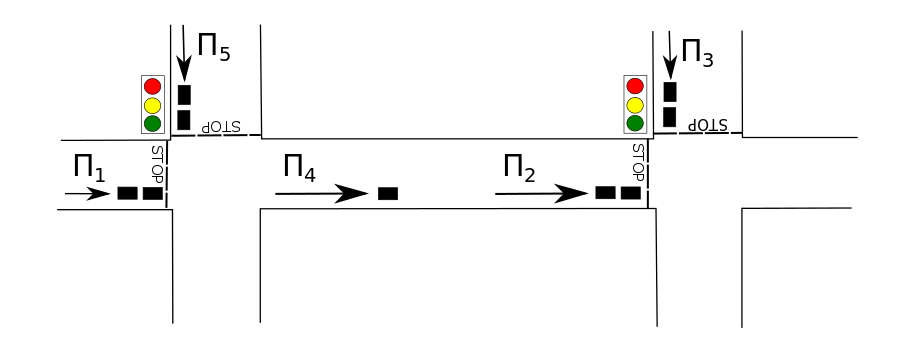
\includegraphics[scale=0.4]{Pictures/Crossroads.png} 
\caption{Пример: тандем перекрестков}
\label{crossroads}
\end{figure}
В качестве наглядной интерпретации системы приводится тандем перекрестков (рис.~\ref{crossroads}). Предполагается, что на первый перекресток поступают автомобили из неординарного пуассоновского потока $\Pi_1$. После прохождения первого перекрестка (обслуживания) эти автомобили формируют поток $\Pi_4$ и, негновенно проезжая расстояние между двумя перекрестками, поступают на второй перекресток, формируя входящий поток $\Pi_2$. На втором перекрестке по циклическому алгоритму с продлением обслуживаются автомобили потоков $\Pi_2$ и $\Pi_3$.

Описанная на содержательном уровне система массового обслуживания должна рассматриваться как абстрактная управляющая система обслуживания. При построении математической модели были выдержаны следующие базовые принципы (принципы кибернетического подхода): принцип дискретности актов функционирования управляющей системы обслуживания во времени; принцип совместного рассмотрения поблочного строения управляющей системы обслуживания и ее функционирования во времени; принцип нелокальности при описании поблочного строения управляющей системы обслуживания. Информация о блоках системы задается с помощью следующих случайных величин и элементов. В качестве дискретной временной шкалы выберем последовательность $\tau_0=0$,  $\tau_1$,  $\tau_2$,  $\ldots$ моментов смены состояния обслуживающего устройства. Обозначим:
1)~$\Gamma_i$,  $i\geqslant 1$,  из множества $\Gamma$~--- состояние обслуживающего устройства в течение времени $\left(\tau_{i-1};\tau_i\right]$ и $\Gamma_0\in \Gamma$~--- в момент времени $\tau_0$;
2)~количество $\varkappa_{j, i} \in \mathbb{Z}_+ $,  $i\geqslant 0$,  требований в очереди $O_j$ в момент времени $\tau_i$;
3)~количество $\eta_{j, i} \in \mathbb{Z}_+$,  $i\geqslant 0$,  требований,  поступивших в очередь $O_j$ по потоку $\Pi_j$ в течение времени $\left(\tau_{i};\tau_{i+1}\right]$;
4)~количество $\xi_{j, i} \in \mathbb{Z}_+$,  $i\geqslant 0$,  требований по потоку насыщения $\Pi^{\mathrm{\text{нас}}}_j$ в течение времени $\left(\tau_{i};\tau_{i+1}\right]$;
5)~количество $\overline{\xi}_{j, i}\in \mathbb{Z}_+$,  $i\geqslant 0$,  реально обслуженных требований по потоку $\Pi_j$ в течение времени $\left(\tau_{i};\tau_{i+1}\right]$; $j=\overline{1, 4}$.

Зависимости между блоками системы задаются следующими функциональными и вероятностными соотношениями. 
Функциональная зависимость
\begin{equation}
\overline{\xi}_{j,  i}=\min\{\varkappa_{j,  i}+\eta_{j,  i},  \xi_{j,  i}\},  \quad j \in \{1,  2,  3\}, 
\label{saturationEq}
\end{equation}
между величиной $\overline{\xi}_{j, i}$ и величинами $\varkappa_{j, i}$,  $\eta_{j, i}$,  $\xi_{j, i}$ реализует стратегию механизма обслуживания требований. Далее,  поскольку 
\begin{equation*}
\varkappa_{j,  i+1}=\varkappa_{j,  i}+\eta_{j,  i}-\overline{\xi}_{j,  i},  \quad  j \in \{1,  2,  3\}, 
\end{equation*}
то из выражения \eqref{saturationEq} следует соотношение
\begin{equation}
\varkappa_{j,  i+1}=\max\{{0,  \varkappa_{j,  i}+\eta_{j,  i}-\xi_{j,  i}}\},  \quad j \in \{1,  2,  3\}.
\label{queuesFunc}
\end{equation}
Из формулировки поставленной задачи следуют соотношения для потока~$\Pi_4$:
\begin{equation}
\eta_{4, i} = \min\{\xi_{1, i},  \varkappa_{1, i}+\eta_{1, i}\},  \quad \varkappa_{4, i+1}=\varkappa_{4, i}+\eta_{4, i}-\eta_{2, i},  \quad \xi_{4, i} = \varkappa_{4, i}.
\label{FourthFunc}
\end{equation}



Пусть $a=(a_1,  a_2,  a_3,  a_4) \in \mathbb{Z}_+^4$ и $x=(x_1,  x_2,  x_3,  x_4) \in \mathbb{Z}_+^4$. Тогда из постановки задачи на содержательном уровне следует,  что при фиксированном значении метки $\nu_i=(\Gamma^{(k,  r)}; x)$ вероятность $\varphi(a,  k,  r,  x)$ одновременного выполнения равенств $\eta_{1,  i}=a_1$,  $\eta_{2,  i}=a_2$,  $\eta_{3,  i}=a_3$,  $\eta_{4,  i}=a_4$ есть 
\begin{equation}
\varphi_1(a_1,  h_T(\Gamma^{(k,  r)},  x_3)) \times \psi(a_2,  x_4,  p_{\tilde{k},  \tilde{r}}) \times \varphi_3(a_3,  h_T(\Gamma^{(k,  r)},  x_3))
\times \delta_{a_4,  \min{\{\ell(\tilde{k},  \tilde{r},  1),  x_1+a_1}\}}, 
\label{conditionProbOne}
\end{equation}
где $\tilde{k}$ и $\tilde{r}$ таковы,  что $\Gamma^{(\tilde{k},  \tilde{r})}=h(\Gamma^{(k,  r)},  x_3)$ и $\delta_{i,  j}$ есть символ Кронекера:
%\begin{equation*}
$$
\delta_{i,  j}=
\begin{cases} 
1, & \quad \text{ если $i=j$, }\\
0, & \quad \text{ если $i\neq j$.}
\end{cases}
$$%\end{equation*}
По своему смыслу $\psi(a_2; x_4, p_{\tilde{k},  \tilde{r}})$ есть вероятность поступления $a_2$ требований по потоку $\Pi_2$ при условии,  что очередь $O_4$ содержит $x_4$ требований и обслуживающее устройство находится в состоянии $\Gamma^{(\tilde{k},  \tilde{r})}$,  так что $u=p_{k,  r}$. При нарушении условия $ 0\leqslant k \leqslant y$ положим $\psi(k; y,  u)$ равной нулю.

Пусть $b=(b_1,  b_2,  b_3,  b_4) \in \mathbb{Z}_+^4$. Из содержательной постановки задачи также следует,  что вероятность $\zeta(b,  k,  r,  x)$ одновременного 
выполнения равенств $\xi_{1,  i}\hm=b_1$,  $\xi_{2,  i}=b_2$,  $\xi_{3,  i}=b_3$,  $\xi_{4,  i}=b_4$ при фиксированном значении $(\Gamma^{(k,  r)}; x)$ метки $\nu_i$ есть
\begin{equation}
\delta_{b_1,  \ell(\tilde{k},  \tilde{r},  1)} \times \delta_{b_2,  \ell(\tilde{k},  \tilde{r},  2)} \times 
\delta_{b_3,  \ell(\tilde{k},  \tilde{r},  3)} \times \delta_{b_4,  x_4}.
\label{conditionProbTwo}
\end{equation}


Основным результатом первой главы является теорема~1, содержательный смысл которой  состоит в том,  что сформулированные выше функциональные связи и вероятностные свойства введенных объектов непротиворечивы и могут быть реализованы на некотором вероятностном пространстве.
%Построим теперь 	вероятностное пространство $(\Omega,  {\mathcal F},  \Pr(\cdot))$,  чтобы можно было рассматривать введеные величины как случайные величины на этом пространстве. А именно,  докажем следующую теорему.

\textbf{Теорема 1.}
Пусть $\gamma_0=\Gamma^{(k_0,  r_0)}\in \Gamma$ и $x^0=(x_{1,  0},  x_{2,  0},   x_{3,  0},  x_{4,  0})\in \mathbb{Z}_+^4$ фиксированы.
Тогда существует вероятностное пространство $(\Omega,   {\mathcal F},   \Pr(\cdot))$ и заданные на нем случайные величины $\eta_{j,  i}=\eta_{j,  i}(\omega)$,   $\xi_{j,  i}=\xi_{j,  i}(\omega)$,   	 $\varkappa_{j,  i}=\varkappa_{j,  i}(\omega)$ и случайные элементы $\Gamma_i=\Gamma_i(\omega)$,   $i\geqslant 0$,   $j\in \overline{1,  4}$,   такие,   что 1) имеют место равенства $\Gamma_0(\omega) = \gamma_0$ и $\varkappa_0(\omega)=x^0$; 2) выполняются соотношения \eqref{gammaFunc},   \eqref{queuesFunc},   \eqref{FourthFunc}; 3) для любых  $a\in \mathbb{Z}_+^4$,   $b\in \mathbb{Z}_+^4$ и любых $x^t=(x_{1,  t},  x_{2,  t},  x_{3,  t},  x_{4,  t}) \in \mathbb{Z}_+^4$,   $\Gamma^{(k_t,  r_t)} \in \Gamma$,   $t = 1,   2,   \ldots$,   таких,   что $\Pr\Bigl(\bigcap\limits_{t=0}^{i}\{\omega\colon \Gamma_t=\Gamma^{(k_t,  r_t)},   \varkappa_t=x^t\}\Bigr)>0$,   условное распределение векторов $\eta_i$ и $\xi_i$,   $i \geqslant 0$,    имеет вид
\begin{multline}
\Pr \Bigl(\{ \omega \colon \eta_i = a,   \xi_i=b\} \,\,\Big
|\bigcap_{t=0}^{i}\{\omega\colon \Gamma_t=\Gamma^{(k_t,  r_t)},   \varkappa_t=x^t\}\Bigr)= \\=
\varphi(a,  k_i,  r_i,  x^i)\times \zeta(b,  k_i,  r_i,  x^i),  
\label{ProbablititiesToProve}
\end{multline}
где функции $\varphi(\cdot,   \cdot,   \cdot,   \cdot)$ и $\zeta(\cdot,   \cdot,   \cdot,   \cdot)$ определяются формулами \eqref{conditionProbOne} и \eqref{conditionProbTwo}.


Исследуемая в работе управляющая система характеризуется следующими объектами:  обслуживающее устройство и очереди $O_1$, $O_2$, $O_3$, $O_4$. Случайная последовательность 
 $\{(\Gamma_i,  \varkappa_{1, i},  \varkappa_{2, i},  \varkappa_{3, i},   \varkappa_{4, i}); i \geqslant 0\}$ служит математическим описанием этих объектов. \underline{\textbf{Вторая глава}} посвящена тем результатам,  которые удается получить для этой пятимерной последовательности, несмотря на ее сложность. А именно, в этой главе доказывается марковость последовательности и проводится классификация ее состояний.

 На основе конструктивно заданного вероятностного пространства (Теорема~1) в  разделе~2.1  строго доказана марковость последовательности  $\{(\Gamma_i,   \varkappa_{i}); i \geqslant 0\}$, где $\varkappa_i = ( \varkappa_{1, i},  \varkappa_{2, i},  \varkappa_{3, i},   \varkappa_{4, i})$. Для этого вводятся вспомогательные множества $
A_i(k_i;r_i;x^i) = \{\omega\colon\Gamma_i=\Gamma^{(k_i, r_i)},  \varkappa_i=x^i\}$, для $i=0$,  $1$,  $\ldots$; здесь  $x^i \in \mathbb{Z}_+^4$,  $k_i=\overline{0;d}$,  $r_i=\overline{1;n_{k_i}}$,  $i=0$,  $1$,  $\ldots$. Тогда для доказательства марковости достаточно показать справедливость равенства
\begin{multline}
\Pr ( A_{i+1}(k_{i+1};r_{i+1};x^{i+1})\, \,  |\cap_{t=0}^{i} A_t(k_t;r_t;x^{t})) = \\ = \Pr ( A_{i+1}(k_{i+1};r_{i+1};x^{i+1})\, \,   |A_i(k_i;r_i;x^{i})),
\label{markovToProve}
\end{multline}
являющегося формальной записью определения марковского свойства последовательности  $\{(\Gamma_i,   \varkappa_{i}); i \geqslant 0\}$. Далее было найдено выражение для переходных вероятностей:

\textbf{Теорема 4.}
Пусть $x$,   $\tilde{x}\in \mathbb{Z}_+^4$ и $\Gamma^{(k,  r)}$,   $\Gamma^{(\tilde{k},  \tilde{r})}=h(\Gamma^{(k,  r)},  x_3) \in \Gamma$. Тогда переходные вероятности однородной счетной марковской цепи $\Mark$ вычисляются по следующей формуле:
\begin{multline}
\Pr (\{\omega\colon \Gamma_{i+1}=\Gamma^{(\tilde{k},  \tilde{r})},  \varkappa_{i+1}=\tilde{x} \}| \{\omega\colon \Gamma_{i}=\Gamma^{(k,  r)},  \varkappa_i=x\})=\\ 
=\widetilde{\varphi}_3(\tilde{k},  \tilde{r},  h_T(\Gamma^{(k,  r)},  x_3),  x_3,  \tilde{x}_3)\times \\ \times
\sum_{(a_1,  a_2)\in {\mathbb A}_{\mathrm{trans}}}\varphi_1(a_1,  h_T(\Gamma^{(k,  r)},  x_3))  \psi(a_2,  x_4,   p_{\tilde{k},  \tilde{r}}).
\label{transitionToProve}
\end{multline}

Аналогичный результат был получен для стохастической последовательности $\MarkThree$: доказана ее марковость и получено выражение для ее переходных вероятностей:

\textbf{Теорема 5.}
Пусть $x_3$,  $\tilde{x}_3\in \mathbb{Z}_+$ и $\Gamma^{(k, r)}\in \Gamma$,  $\Gamma^{(\tilde{k}, \tilde{r})}=h(\Gamma^{(k, r)}, x_3) \in \Gamma$. Тогда переходные вероятности однородной счетной марковской цепи $
\MarkThree
$
вычисляются по следующей формуле:
\begin{multline}
\Pr (\{\omega\colon\Gamma_{i+1}=\Gamma^{(\tilde{k}, \tilde{r})}, \varkappa_{3, i+1}=\tilde{x}\}|\{\omega\colon\Gamma_{i}=\Gamma^{(k, r)}, \varkappa_{3, i}=x\}) 
= \\ =\widetilde{\varphi}_3(\tilde{k}, \tilde{r}, h_T(\Gamma^{(k, r)}, x_3), x_3, \tilde{x}_3).
\label{transitionToProve:three}
\end{multline}
 
 В разделе~2.2  проведена классификация состояний марковской цепи $\Mark$  по арифметическим свойствам переходных вероятностей и выделено множество ее существенных состояний. Данный шаг является необходимым для изучения асимптотических свойст абстрактной управляющей системы. Результатом этого шага является следующая теорема.
 
 \textbf{Теорема 6.}
Состояния вида
$(\Gamma^{(\tilde{k}, \tilde{r})}, \tilde{x})$, 
где $\tilde{k}=\overline{0, d}$,  $\tilde{r} = \overline{1, n_{\tilde{k}}}$,  $\tilde{x}\in \mathbb{Z}_+^4$, 
\begin{gather}
(\tilde{x}_1>0) \Rightarrow (\tilde{x}_4\geqslant \ell(\tilde{k}, \tilde{r}, 1)), \label{reachable:1}\\
\tilde{x}_3\geqslant \max{\Bigl\{0, L+1-\sum_{s=1}^{\tilde{r}}\ell(k, s, 3)\Bigr\}},  \text{ если } \tilde{k}>0, \\
\tilde{x}_3\geqslant \max{\Big\{0, L+1-\max_{k=\overline{1, d}}{\{\sum_{s=1}^{n_{\tilde{k}}} \ell(\tilde{k}, s, 3)\}}\Bigr\}},  \text{ если } \tilde{k}=0, \label{reachable:2}
\end{gather}
 и только они достижимы из состояния 
 $$
 (\Gamma^{(0,  r_0)},  x^0),  \quad x^0=(0,  0,  L+1,  0),  \quad r_0=\overline{1, n_0}, 
 $$ и,  следовательно,  являются существенными.

Доказательство этой теоремы начинается с выделения наиболее очевидных существенных состояний (леммы~1--3):
$$(\Gamma^{(0,  r_0)},  \tilde{x}),  \quad r_0 = \overline{1,  n_0},  \tilde{x}=(0,  0,  L+1,  0).$$ Затем это множество постепенно расширяется (леммы~4--9).

Из доказанных результатов также находятся существенные состояния для марковской цепи $\MarkThree$:

\textbf{Теорема 7.}
Множество существенных состояний марковской цепи $\MarkThree$ имеет вид $\raisebox{-.5ex}{$\Bigl($}\bigcup\limits_{1 \leqslant r \leqslant n_0}S^3_{0, r}\raisebox{-.5ex}{$\Bigr)$}\cup \raisebox{-.5ex}{$\Bigl($}\bigcup\limits_{\substack{1 \leqslant k \leqslant d\\ 1 \leqslant r \leqslant n_k}} S^3_{k, r}\raisebox{-.5ex}{$\Bigr)$}$,
где
\begin{align*}
  S^3_{0, r} = & 
  \Bigl\{
  (\Gamma^{(0,  r)},  x_3) \colon \; x_3\in Z_+, \; x_3 > L - \max\limits_{k=1,  2, 
    \ldots,  d}
  \Bigl\{ \sum_{t=1}^{n_k} \ell({k,  t,  3}) \Bigl\}\Bigl\},  
   1 \leqslant r \leqslant n_0,  \\
  S^3_{k,  r} = & 
  \Bigl\{
  (\Gamma^{(k,  r)},  x_3) \colon \; x_3\in Z_+, \; x_3 > L - \sum_{t=1}^{r} \ell({k,  t,  3})
  \Bigr\},  
   1 \leqslant k \leqslant d,  \quad 1 \leqslant r \leqslant n_k.
\end{align*}

 Результаты этой главы позволяют доказать марковость и провести классификацию состояний для последовательностей,  содержащих только часть из упомянутых пяти компонент (содержащих только часть очередей).
 


В  \underline{\textbf{третьей главе}} более подробно изучаются случайные последовательности,  содержащие состояния только части очередей из последовательности $\Mark$: очереди $O_1$, $O_3$ и $O_4$. Исключение из рассмотрения нескольких компонент пятмерной марковской цепи позволяет найти достаточное, а в некоторых случаях  необходимое условия существования стационарного распределения. 

Начинается глава с раздела~3.1, в котором рассматривается стохастическая последовательность $\{\varkappa_{4, i}(\omega); i =0,  1,  \ldots\}$, не являющаяся, вообще говоря, марковской. Дело в том, что в силу определенных условий, для решения вопроса существования стационарного распределения для общей последовательности $\Mark$ достаточно доказать ограниченность отдельных ее компонент. Поэтому, ограниченность последовательности $\{\varkappa_{4, i}(\omega); i =0,  1,  \ldots\}$ представляет собой важный вопрос.

\textbf{Теорема 8.}
Для того,  чтобы последовательность 
$
\{\varkappa_{4, i}(\omega); i =0,  1,  \ldots\}, 
$ была ограничена,  достаточно выполнения неравенства
$
   % \min_{\substack{k=\overline{1, d}\\ j=1, 3}} {\{p_{k, r}\}} > 0.
    \min_{k=\overline{0, d},  r=\overline{1, n_k}} {\{p_{k, r}\}} > 0.
$

Для нахождения условий стационарности используется хорошо зарекомендовавший себя в схожих задачах итеративно-мажорантный метод,  в котором последовательность математических ожиданий отдельных компонент цепи $\Mark$ ограничивается числовой последовательностью более простого вида. С этой целью в разделе~3.2 выводятся рекуррентные соотношения для производящих функций последовательности $\MarkThree$.

Более подробно, пусть $\Gamma^{(k, r)}\in \Gamma$ и $x_3 \in {\mathbb Z}_+$. Обозначим 
\begin{equation*}
{\mathbb H}_{-1}(\Gamma^{(k, r)},  x_3) = \{\gamma \in \Gamma \colon h(\gamma,  x_3) = \Gamma^{(k, r)}\}.
\end{equation*}


\textbf{Теорема 10.}
Пусть $\tilde{\gamma}=\Gamma^{(\tilde{k}, \tilde{r})} \in \Gamma$. Тогда имеют место следующие рекуррентные по $i \geqslant 0$ соотношения для производящих функций $\mathfrak{M}^{(3, i+1)}(\cdot, \cdot, v)$ марковской цепи $\MarkThree$:
\begin{enumerate}
\item для $ \Gamma^{(0, \tilde{r})} \in \Gamma$,  $\tilde{r} = \overline{1, n_0}$ 
\begin{equation}
\mathfrak{M}^{(3, i+1)}(0, \tilde{r}, v) = \alpha_i(0, \tilde{r}, v);
\label{three:generation:rek:one}
\end{equation}
\item для $\Gamma^{(\tilde{k}, \tilde{r})} \in \Gamma $,  $\tilde{k} =\overline{1, d}$,  $\tilde{r}=\overline{1, n_{\tilde{k}}}$
\begin{equation}
\mathfrak{M}^{(3, i+1)}(\tilde{k}, \tilde{r}, v) = q_{\tilde{k}, \tilde{r}} (v)\times  \mathfrak{M}^{(3, i)}(\tilde{k}, \tilde{r} \ominus_{\tilde{k}} 1, v) + \alpha_i(\tilde{k}, \tilde{r}, v).
\label{three:generation:rek:two}
\end{equation}
\end{enumerate}

Поскольку математическое ожидание случайной величины очевидным бразом связано с производящей функцией, то имея в арсенале рекуррентные соотношения для производящих функций последовательности $\MarkThree$, теперь можно применить итеративно-мажорантный метод для поиска достаточного условия существования стационарного распределения $Q_{3, i}(\gamma, x)$.

% Обозначим для $\gamma \in \Gamma$ и $x_3 \in {\mathbb Z}_+$
% \begin{equation}
% Q_{3, i}(\gamma, x) = \Pr(\Gamma_{i}=\gamma,  \varkappa_{3, i}=x_3).
% \end{equation}

\textbf{Теорема 11.}
Для того,  чтобы марковская цепь $\MarkThree$ имела стационарное распределение $Q(\gamma, x)$,  $(\gamma, x)\in \Gamma \times {\mathbb Z}_+$, достаточно выполнения неравенства 
\begin{equation}
\min_{k=\overline{1, d}} { \frac{\sum_{r = 1}^{n_k} \ell(k, r, 3) }{\lambda_3 f_3'(1) \sum_{r=1}^{n_k} T^{(k, r)} }}>1.
\label{sufficient:low}
\end{equation}
Доказательство этого факта осуществляется от противного и здесь мы приведем лишь основную идею. Пусть при выполнении условий \eqref{sufficient:low} стационарного распределения не существует.  
Тогда для любого состояния $(\gamma, x)\in \Gamma \times {\mathbb Z}_+$ и независимо от начального распределения $\Pr(\Gamma_{0}=\Gamma^{(k, r)},  \varkappa_{3, 0}=x)$, 
$(\Gamma^{(k, r)}, x)\in \Gamma \times {\mathbb Z}_+$,  
имеют место предельные равенства 
\begin{equation}
\lim_{i \to \infty} \Pr(\Gamma_{i}=\Gamma^{(k, r)},  \varkappa_{3, i}=x) =0,  \quad  (\Gamma^{(k, r)}, x)\in \Gamma \times {\mathbb Z}_+.
\label{zero:limit:equations}
\end{equation} 
Для доказательства этого факта достаточно рассмотреть все возможные случаи,  предполагая апериодичность рассматриваемой цепи:
\begin{enumerate}
\item все состояния цепи $\MarkThree$ невозвратные,  тогда предельные соотношения выполняются;
\item существует хотя бы одно возвратное состояние,  тогда все состояния возвратные (поскольку все состояния сообщающиеся); и пусть все состояния нулевые,  тогда предельное соотношение также выполняется;
\item все состояния возвратные и существует хотя бы одно положительное,  тогда все состояния положительные и пределы 
$$
\lim_{i \to \infty} \Pr(\Gamma_{i}=\Gamma^{(k, r)},  \varkappa_{3, i}=x) > 0
$$
являются стационарными вероятностями, что противоречит предположению.
\end{enumerate}
Для периодической цепи приведенные рассуждения достаточно провести для циклических подклассов.

Далее показывается, что из соотношений \eqref{zero:limit:equations} следует неограниченность математических ожиданий $E[\varkappa_{3,i}]$ при $i \to \infty$. Однако, возможно построить такую последовательность $\mathfrak{M}_+^{(3, 0)}(k, r, v)$, которая была бы мажорантой для соответствующих исходных производящих функций $\mathfrak{M}^{(3, 0)}(k, r, v)$ в некоторой окрестности точки $v=1$. Для мажорирующей последовательности, в силу ее меньшей сложности, удается доказать  равномерную по $i$ ограниченность и, применяя интегральную формулу Коши, доказать ограниченность и ее производной. В следствие вышесказанного, математические ожидания $E[\varkappa_{3,i}]$ также являются ограниченными и в силу противоречия получается утверждение теоремы. 

В разделе~3.4 в качестве необходимого условия существования стационарного распределения доказывается менее строгое условие. Оно сформулированно в следующей теореме.

\textbf{Теорема 12.}
Для того,  чтобы марковская цепь $\MarkThree$ имела стационарное распределение $Q_3(\gamma, x)$,  $(\gamma, x)\in \Gamma \times {\mathbb Z}_+$,  необходимо выполнение неравенства
$$
\max_{k=\overline{1, d}} { \frac{\sum_{r = 1}^{n_{k}}\ell(k, r, 3)}{\lambda_3 f_3'(1) \sum_{r = 1}^{n_k} T^{(k, r)}} } >1.
$$

Доказательство в данном случае основывается на том свойстве частичных производящих функций $\mathfrak{M}^{(3, i)}(k, r, v)$, что при суммировании при $v=1$ по $k$ и $r$ они дают $1$. Поэтому складывая известные рекуррентные соотношения для $\mathfrak{M}^{(3, i)}(k, r, v)$, появляется необходимое условие на параметры системы.

Раздел~3.5 содержит достаточное условие существования стационарного распределения для последовательности $\{(\Gamma_i,  \varkappa_{1, i}, \varkappa_{3, i}); i \geqslant 0\}$, доказательство которого проводится при помощи итеративно-мажорантного метода аналогично результату для последовательности $\MarkThree$.

\textbf{Теорема 16.}
Для того,  чтобы марковская цепь $\{(\Gamma_i,  \varkappa_{1, i}, \varkappa_{3, i}); i \geqslant 0\}$ имела стационарное распределение $Q_1(\gamma, x_1, x_3)$,  $(\gamma, x_1, x_3)\in \Gamma \times {\mathbb Z}^2_+$,  достаточно выполнения неравенств
\begin{equation}
\min_{k=\overline{0, d}} { \frac{\sum_{r = 1}^{n_k} \ell(k, r, 1) }{\lambda_1 f_1'(1) \sum_{r=1}^{n_k} T^{(k, r)} }}>1,  \quad 
\min_{k=\overline{1, d}} { \frac{\sum_{r = 1}^{n_k} \ell(k, r, 3) }{\lambda_3 f_3'(1) \sum_{r=1}^{n_k} T^{(k, r)} }}>1.
\end{equation}


 \underline{\textbf{Четвертая глава}} имеет своей целью проанализировать и расширить результаты, полученные аналитически в предыдущих главах. Поэтому здесь представлено описание разработанной имитационной модели и программного комплекса для ее исследования. Для определения момента достижения системой стационарного режима подсчитываются различные статистики одновременно для двух систем: смещенной, то есть системы с ненулевым количеством требований в начале, и несмещенной, то есть системы с пустыми очередями при старте. Основным показателем качества работы системы выбрана средневзвешенная оценка времени пребывания требования в системе. В завершении главы приведены конкретные эксперименты и анализ их результатов.





Комплексные системы, состоящие из нескольких схожих или различных подсистем, могут рассматриваться с точки зрения понятия <<сложная система>>. Общее определение <<сложной системы>> было введено в работе \cite{Buslenko:1978} на основе изучения большого количества реальных комплексных систем и их математических моделей. Для анализа подобных систем ранее использовался весьма широкий математический аппарат: конечные автоматы, дифференциальные уравнения, динамические системы и теория массового обслуживания. Поэтому введение единого общего понятия представлялось актуальным и было осуществлено именно в работе \cite{Buslenko:1978}. Тандем управляющих систем обслуживания является одним из примеров таких <<сложных систем>>. 

До этой главы в работе исследовались свойства основных подсистем тандема: подсистемы с очередью низкоприоритетного потока, с очередями первичных входных потоков и с промежуточной очередью. Тем не менее, для всестороннего изучения системы необходимо также провести ее синтез. Другими словами, здесь и далее нас будет интересовать поведение системы в целом: ее эффективность и устойчивость с течением времени. Эффективность подобных систем может оцениваться, к примеру, с помощью одной из следующих характеристик: 1) среднее взвешенное количество ожидающих требований в очередях; 2) среднее взвешенное время нахождения в системе произвольного требования; 3) среднее взвешенное время ожидания в системе произвольного требования; 4) среднее время простоя системы. В данной работе акцент будет сделан на среднем взвешенном времени ожидания и средем взвешенном времени пребывания произвольного требования в системе.

% На базе математической модели тандема управляющих систем обслуживания построена имитационная модель для двух перекрестков (рис.~\ref{../Pictures/Crossroads.png}).

Математическая модель рассматриваемой в работе абстрактной управляющей системы Ляпунова--Яблонского, построенная по принципам кибернетического подхода, существенно упростила построение и реализацию имитационной модели тандема перекрестков (рис.~\ref{crossroads}). В частности, нелокальное описание блоков системы помогло избежать формирования большого количества данных и, как следствие, их последующей обработки. Время имитации при этом должно существенно сократиться. Для смещенной и несмещенной систем в роли состояния выступали длины очередей и состояние обслуживающего устройства. В соответствии с законами распределения входных потоков  $\Pi_1$ и $\Pi_3$ генерировались требования системы. Для каждого требования фиксировался момент его прихода в систему, выхода из нее и время до обслуживания.

Альтернативным подходом к изложенному в этой работе является метод дискретных событий. В противовес нелокальному описанию системы, в роли наблюдаемых событий, как правило, выбирались вход в систему или выход из нее конкретного требования, момент смены обслуживающим устройством его состояния и т.д. В результате формируется исчерпывающее множество событий системы и создается полное описание всего процесса обслуживания. Поскольку для получения оценки основных характеристик работы системы такой объем информации является избыточным, то представляется целесообразным и зачастую необходимым отказаться от большей ее части.

В настоящей работе наибольший акцент при оценке эффективности работы системы делается на среднее взвешенное время нахождения произвольного требования первичных потоков $\Pi_1$ и $\Pi_3$ в системе: чем больше средняя интенсивность потока требований, тем больше вес требований этого потока. Время ожидания требований первичных потоков не характеризует процессов, происходящих между двумя перекрестками, поэтому в качестве конечного критерия эффективности работы не используется. Размер каждой очереди $O_j$, $j=\overline{1,4}$, сложно преобразовать в единую характеристику, поскольку очереди имеют качественно разную природу. Однако для определения момента наступления стационарного режима данная информация оказывается весьма полезной.




 В \underline{\textbf{заключении}} приведены основные результаты работы, которые заключаются в следующем.

    \begin{enumerate}
        \item Построена строгая математическая модель тандема с циклическим алгоритмом управления и алгоритмом с продлением. Отличительной особенностью системы также является немгновенность перемещения требований между системами. 
        \item Доказана марковость случайной последовательности, включающей длину низкоприоритетной очереди. Проведена классификация состояний цепи по арифметическим свойствам переходных вероятностей этой последовательности. А также найдены достаточное и необходимое условия существования стационарного распределения.
        \item Проведен аналогичный анализ для случайной последовательности, включающей очереди первичных требований: доказана ее марковость, проведена классификация состояний и найдено достаточное условие существования стационарного распределения.
        \item Найдено условие ограниченности для последовательности математических ожиданий $    \{( E\varkappa_{4,i}); i \geqslant 0\}$.
%        \item Разработана имитационная модель для изучения исходной системы и написана программа ее реализующая.
        \item На основе имитационной модели расширены результаты, полученные теоретически.
    \end{enumerate}














\section*{Список публикаций по теме диссертации}

\textbf{Публикации в изданиях, рекомендованных ВАК Российской Федерации и включенных в перечень международных баз цитирования (Web of Science, Scopus):}
\begin{enumerate}
\item Kocheganov~V.M., Zorine~A.V. Low-priority queue fluctuations in tandem of queuing systems under cyclic control with prolongations // Communications in Computer and Information Science~--- Vol.~601.~--- 2016.~--- Pp.~268--279.
\item Kocheganov~V.M., Zorine~A.V. Low-priority queue and server's steady-state existence in a tandem under prolongable cyclic service // Communications in Computer and Information Science.~--- V.~678.~--- 2016.~--- Pp.~210--221.
\item  Кочеганов~В.М., Зорин~А.В. Статистический анализ и оптимизация тандема систем массового обслуживания в классе циклических алгоритмов с продлением // Управление Большими Системами: сборник трудов.~--- 2019.~--- №~78.~--- С.~122~--148.
\item Кочеганов~В.М., Зорин~А.В. Достаточное условие существования стационарного режима очередей первичных требований в тандеме систем массового обслуживания // Вестник ТвГУ. Серия: Прикладная математика.~--- 2018.~--- №~2.~--- С.~49--74.
\item
 Кочеганов~В.М. Классификация состояний марковской цепи в модели тандема с циклическим управлением с продлением // Известия Саратовского университета. Новая серия. Серия Математика. Механика. Информатика.~--- 2020.~--- Т.20~--- В.2.~--- С.~257--265.
\end{enumerate}	

\textbf{Свидетельство о государственной регистрации программы для ЭВМ:}
\begin{enumerate}[resume]
	\item Кочеганов~В.М. Статистический анализ тандема перекрестков с циклическим алгоритмом и алгоритмом с продлением: А. с. №~2019612786, дата государственной регистрации в Реестре программ для ЭВМ 27 февраля
2019 г.~--- 2019.
\end{enumerate}

\pagebreak
\textbf{Публикации в изданиях, рекомендованных ВАК Российской Федерации для защиты по смежным специальностям:}

\begin{enumerate} 	[resume]
\item Кочеганов~В.М., Зорин~А.В. Достаточное условие существования стационарного режима низкоприоритетной очереди в тандеме систем массового обслуживания // Вестник Волжской государственной академии водного транспорта.~--- 2017.~--- №~50.~--- С.~47--55.
\item Кочеганов~В.М. Анализ тандема систем
массового обслуживания с циклическим управлением с продлением // Теория вероятностей и ее применения.~--- М.: Наука, 2020.~--- Т.65~--- В.1~--- С.~169--170.
\end{enumerate}	

\textbf{Публикации в иных научных изданиях:}

\begin{enumerate}[resume]
  \item Кочеганов~В.М., Зорин~А.В. Вероятностная модель тандема систем массового обслуживания с циклическим управлением с продлением // Теория вероятностей, случайные процессы, математическая статистика и приложения. Материалы Международной научной конференции.~--- Минск:~РИВШ, 2015~--- С.~94--99.
\item Кочеганов~В.М., Зорин~А.В. Дискретная модель колебания длины низкоприоритетной очереди в тандеме систем массового обслуживания при циклическом алгоритме с продлением // IX Международная конференция <<Дискретные модели в теории управляющих систем>>: Москва и Подмосковье, 20--22 мая 2015~г.: Труды / Отв. ред. В.Б.~Алексеев, Д.С.~Романов, Б.Р.~Данилов.~--- М:~МАКС Пресс, 2015.~--- С.~126--129.
\item Kocheganov~V.M., Zorine~A.V. Low-priority queue fluctuations in tandem of queuing systems under cyclic control with prolongations // Распределенные компьютерные и телекоммуникационные сети: управление, вычисление, связь (DCCN-2015): материалы Восемнадцатой международной научной конференции.~--- М.: ИПУ РАН, 2015.~--- С.~136--143.
\item Kocheganov~V.M., Zorine~A.V. Low-priority queue and server’s steady-state existence in a tandem under prolongable cyclic service // Распределенные компьютерные и телекоммуникационные сети: управление, вычисление, связь (DCCN-2016): материалы Девятнадцатой международной научной конференции: в 3 томах, под общей редакцией В.М.~Вишневского и К.Е.~Самуйлова.~--- М.: РУДН, 2016.~--- С.~232--239.
\item Кочеганов~В.М., Зорин~А.В. Анализ потоков первичных требований в тандеме при циклическом управлении с продлением // Информационные технологии и математическое моделирование (ИТММ--2017). Материалы XVI Международной конференции имени А.Ф. Терпугова (29 сентября -- 3 октября 2017 г.).~--- Т.~1.~--- Томск: Изд-во~НТЛ.~--- 2017.~--- С.81--87.
\item Кочеганов~В.М., Зорин~А.В. Изучение процесса управления потоками первичных требований в тандеме систем обслуживания с циклическим алгоритмом с продлением // Проблемы теоретической кибернетики: XVIII международная конференция (Пенза, 19--23 июня 2017~г.). Материалы: под редакцией Ю.И.~Журавлева.~--- М.:~МАКС~Пресс, 2017.~--- С.~135--137.
\item Kocheganov~V., Zorine~A. Primary input flows in a tandem under prolongable cyclic service // Распределенные компьютерные и телекоммуникационные сети: управление, вычисление, связь (DCCN-2017). Материалы Двадцатой международной научной конференции: под общ. ред. В.М. Вишневского.~--- М:~ТЕХНОСФЕРА, 2017.~--- Pp.~517--525.
\item Kocheganov~V., Zorine~A. Asymptotic properties of service and control operations in tandem systems with cyclic algorithms with prolongation //IX Moscow International Conference on Operations Research (ORM-2018).~--- Vol.~1.~---2018. ~--- Pp.~337--342
\item  Кочеганов~В.М. Классификация состояний марковской цепи в модели тандема с циклическим управлением с продлением // Информационные технологии и математическое моделирование (ИТММ-2019). Материалы
XVIII Международной конференции имени А.Ф. Терпугова (26 июня -- 30 июня 2019 г.).~--- Томск: Изд-во~НТЛ, 2019.~--- С.~195~--200.
\end{enumerate}	

